\section{Introduction}
\begin{frame}{Introduction}
    \begin{itemize}
        \item \textbf{Goal:} Identification and quantification of chemical elements on the lunar surface to support future exploration.
        \item \textbf{The Challenge:} Remote sensing via X-ray Fluorescence (XRF) produces complex, noisy, and high-dimensional spectral data.
        \item \textbf{Methodology:} Using Machine Learning to automate and refine the interpretation of these spectra.
        \item \textbf{Data Strategy:} Development of a custom dataset and utilization of \texttt{multiel-spectra} for high-fidelity synthetic data generation.
    \end{itemize}
\end{frame}

\begin{frame}{XRF Spectroscopy Fundamentals}
    \begin{columns}
        \column{0.5\textwidth}
        \begin{itemize}
            \item High-energy X-rays/Gamma rays irradiate the sample.
            \item Secondary X-rays (fluorescence) are emitted, unique to each element.
            \item The detector captures a spectrum where energy peaks correspond to specific atoms.
        \end{itemize}
        \column{0.5\textwidth}

        \begin{figure}
            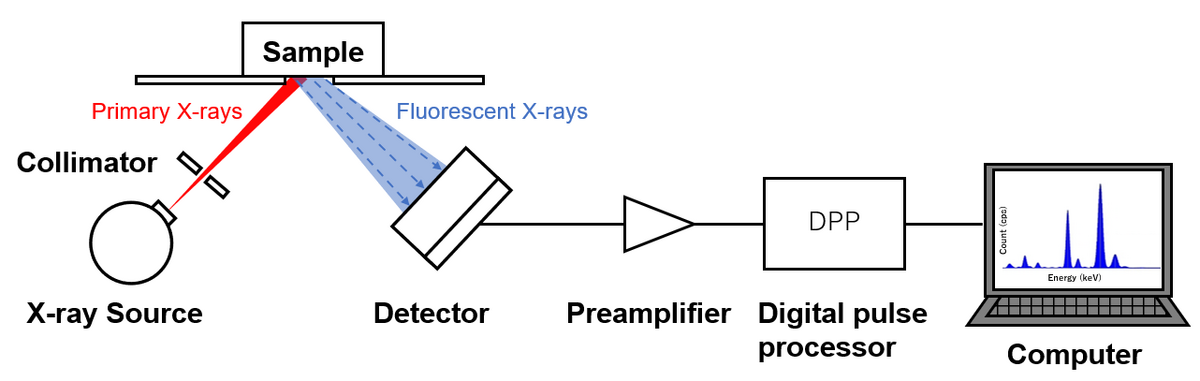
\includegraphics[width=\linewidth]{media/xrf_diagram.png}
        \end{figure}

    \end{columns}
\end{frame}